\documentclass{beamer}
  \usepackage[czech]{babel}
  \usepackage[utf8]{inputenc}
  \usepackage[T1]{fontenc}
  \usepackage{textcomp}
  \usepackage{color}

  \usetheme{Boadilla}
  \usecolortheme{beaver}

  \title[IFJ12]{Implementace interpretu imperativního jazyka IFJ12}
  \subtitle{Tým 034, varianta a/1/II}
  \author[Tým 034]{Michal Duban \and Marko Fábry \and Václav Hanselka \and Petra Hecková \and Jan Wrona}
  \institute[FIT VUT]{Vysoké učení technické v Brně}

\begin{document}
\frame{\titlepage}

\begin{frame}{Struktura interpretu}
  \begin{center}
    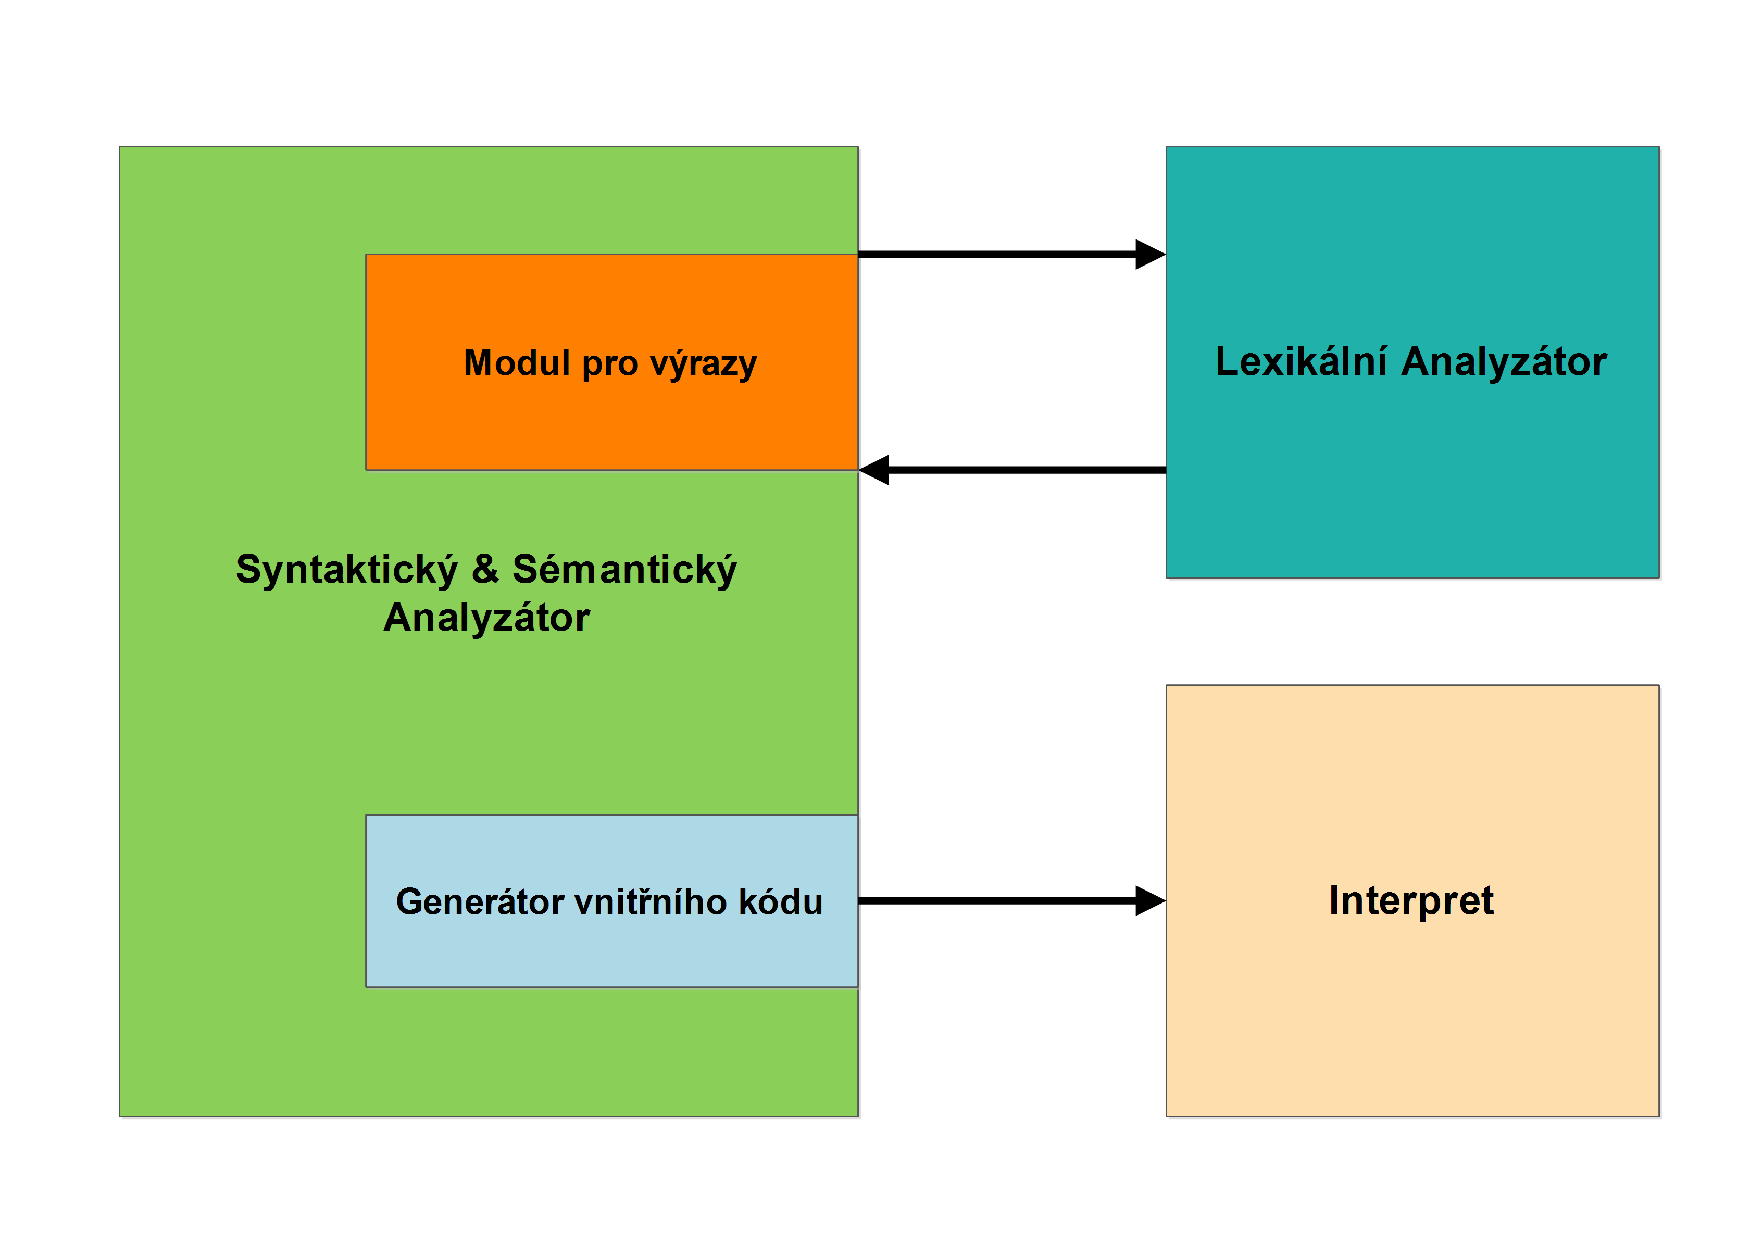
\includegraphics[trim=0 0 0 20px, scale=0.38]{struktura.pdf}
  \end{center}
\end{frame}

\begin{frame}{Struktura FSM}
  \begin{center}
    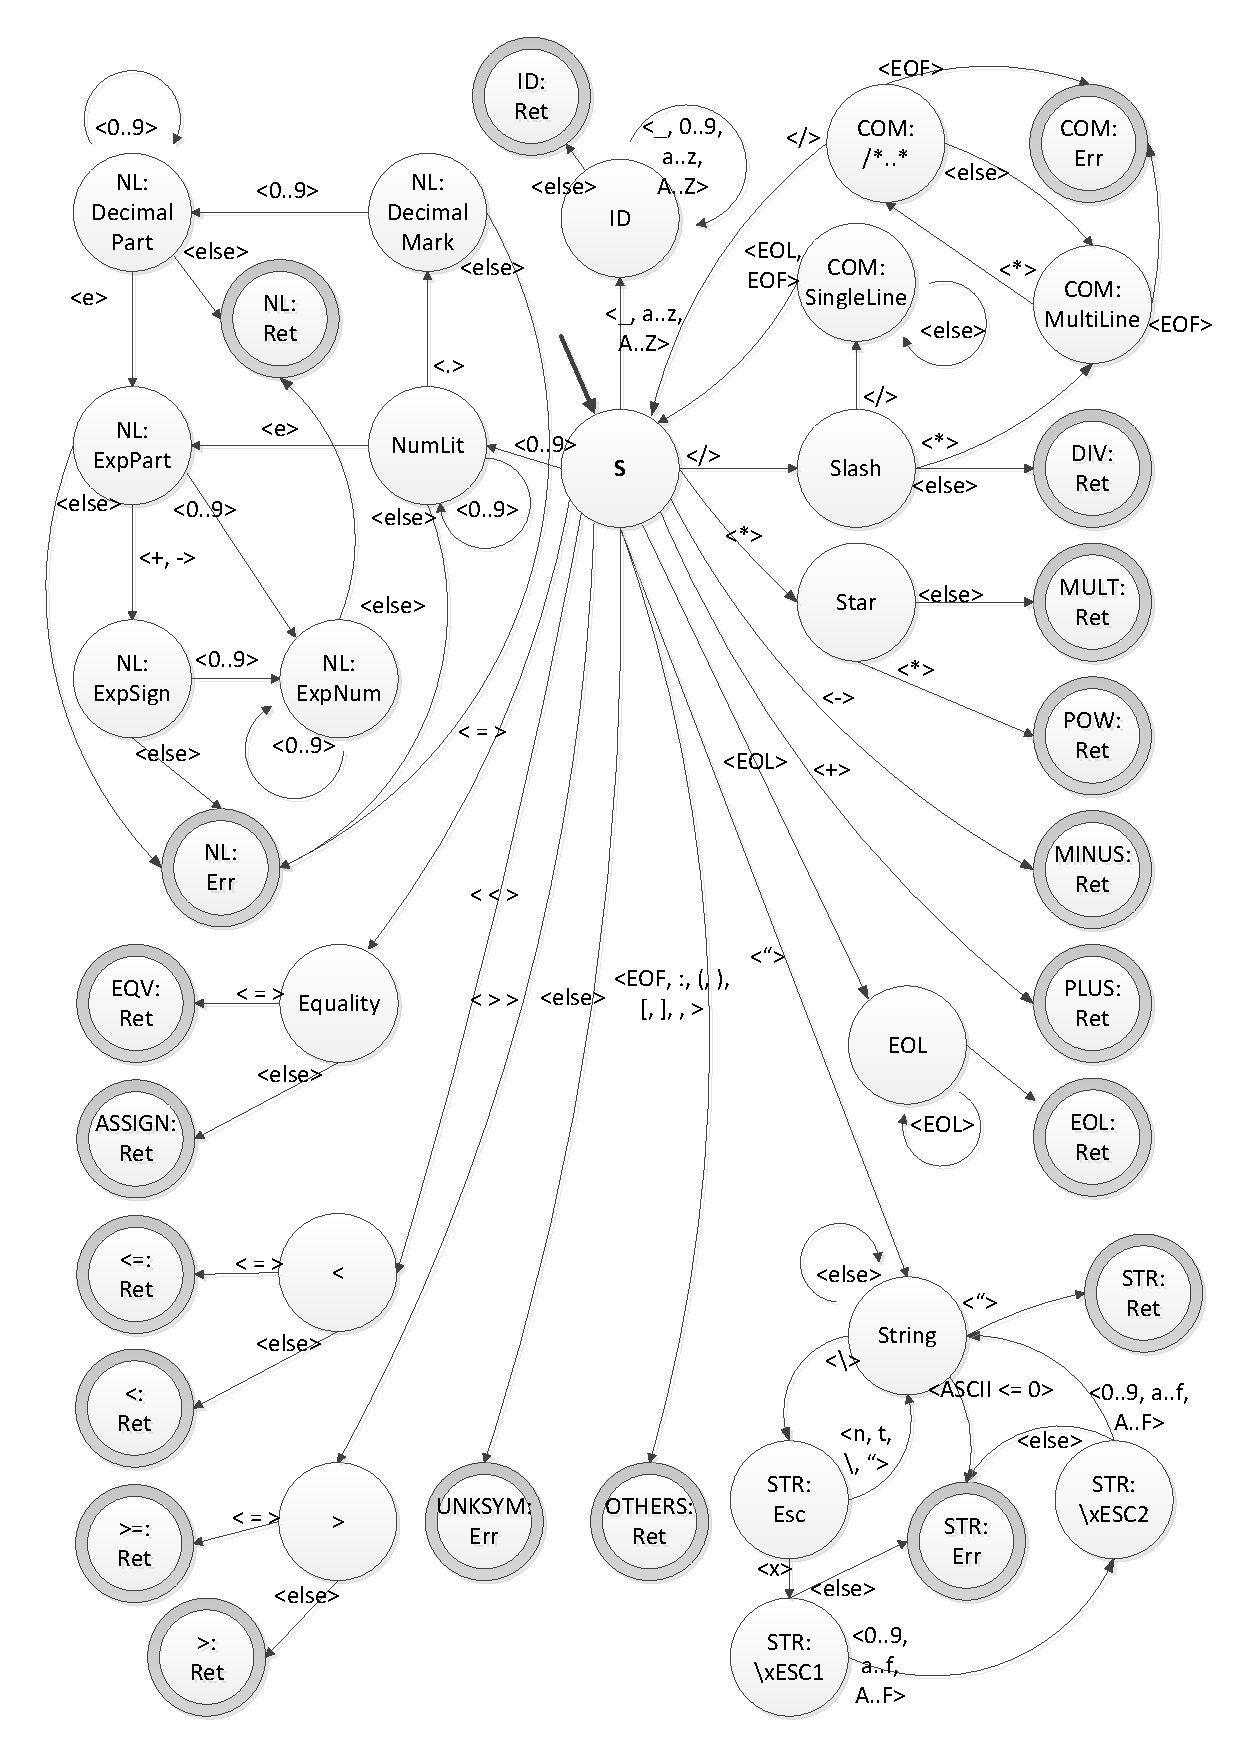
\includegraphics[scale=0.25]{fsm.pdf}
  \end{center}
\end{frame}

\begin{frame}{LL gramatika pro programové konstrukce}
  \begin{enumerate}
  {\footnotesize
  \item {<program>\textrightarrow<statementlist>}
  \item {<statementlist>\textrightarrow<statement> <statementlist>}
  \item {<statementlist>\textrightarrow<statement>}
  \item {<statement>\textrightarrow EOF}
  \item {<statement>\textrightarrow IF<e>EOL<statementlist>ELSE EOL<statementlist>END EOL}
  \item {<statement>\textrightarrow IDENT = <e> EOL}
  \item {<statement>\textrightarrow IDENT = IDENT( <arglist> EOL}
  \item {<statement>\textrightarrow WHILE <e> EOL <statementList> END EOL}
  \item {<statement>\textrightarrow RETURN <e> EOL}
  \item {<statement>\textrightarrow FUNCTION IDENT ( <arglist> EOL <statementlist> END EOL}
  \item {<arglist>\textrightarrow )}
  \item {<arglist>\textrightarrow IDENT , <arglist>}
  \item {<arglist>\textrightarrow IDENT )}
  }
  \end{enumerate}
\end{frame}

\begin{frame}{Pravidla pro zpracování výrazů}
  \begin{enumerate}
  {\footnotesize
  \item {<e>\textrightarrow IDENT}
  \item {<e>\textrightarrow ( <e> )}
  \item {<e>\textrightarrow <e> ** <e>}
  \item {<e>\textrightarrow <e> * <e>}
  \item {<e>\textrightarrow <e> / <e>}
  \item {<e>\textrightarrow <e> +<e>}
  \item {<e>\textrightarrow <e> -<e>}
  \item {<e>\textrightarrow <e> == <e>}
  \item {<e>\textrightarrow <e> != <e>}
  \item {<e>\textrightarrow <e> <= <e>}
  \item {<e>\textrightarrow <e> >= <e>}
  \item {<e>\textrightarrow <e> < <e>}
  \item {<e>\textrightarrow <e> > <e>}
  \item {<e>\textrightarrow IDENT [IDENT : IDENT]}
  }
  \end{enumerate}
\end{frame}

\begin{frame}{Knuth–Morris–Prattův algoritmus}
  \begin{itemize}
    \item výhoda: nevrací se k již prohledaným znakům
  \end{itemize}
  \begin{center}
  \begin{tabular}{|l|@{}c@{}|@{}c@{}|@{}c@{}|@{}c@{}|@{}c@{}|@{}c@{}|@{}c@{}|@{}c@{}|@{}c@{}|@{}c@{}|@{}c@{}|@{}c@{}|@{}c@{}|@{}c@{}|@{}c@{}|@{}c@{}|@{}c@{}|@{}c@{}|@{}c@{}|}
  \hline
     &0&1&2&3&4&5&6&7&8&9&0&1&2&3&4&5&6&7&8\\ \hline
     &A&B&C&D&A&B& &A&B&C&D&A&B&C&D&A&B&D&E\\ \hline
    1.&A&B&C&D&A&B&\textcolor{red}{D}& & & & & & & & & & & & \\ \hline
    2.& & & & &A&B&\textcolor{red}{C}&D&A&B&D& & & & & & & & \\ \hline
    3.& & & & & & & &A&B&C&D&A&B&\textcolor{red}{D}& & & & & \\ \hline
    4.& & & & & & & & & & & &A&B&C&D&A&B&\textcolor{green}{D}& \\ \hline
  \end{tabular}
  \end{center}
\end{frame}

\begin{frame}{Quicksort}
  \begin{itemize}
    \item volba pivotu
    \item využití rekurze
    \item průměrná složitost $O(N\ log_2\ N)$
    \item nejhorší složitost $O(N^2)$
  \end{itemize}
  \begin{center}
    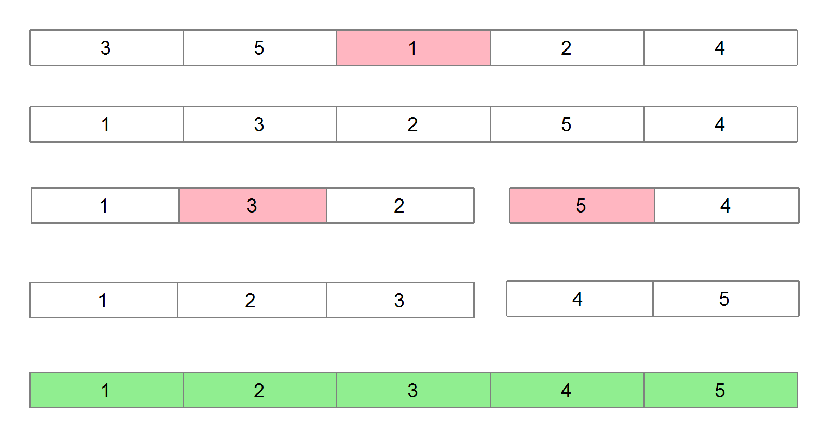
\includegraphics[scale=0.5]{qs.pdf}
  \end{center}
\end{frame}

\begin{frame}{Popis datových struktur}
  \begin{center}
    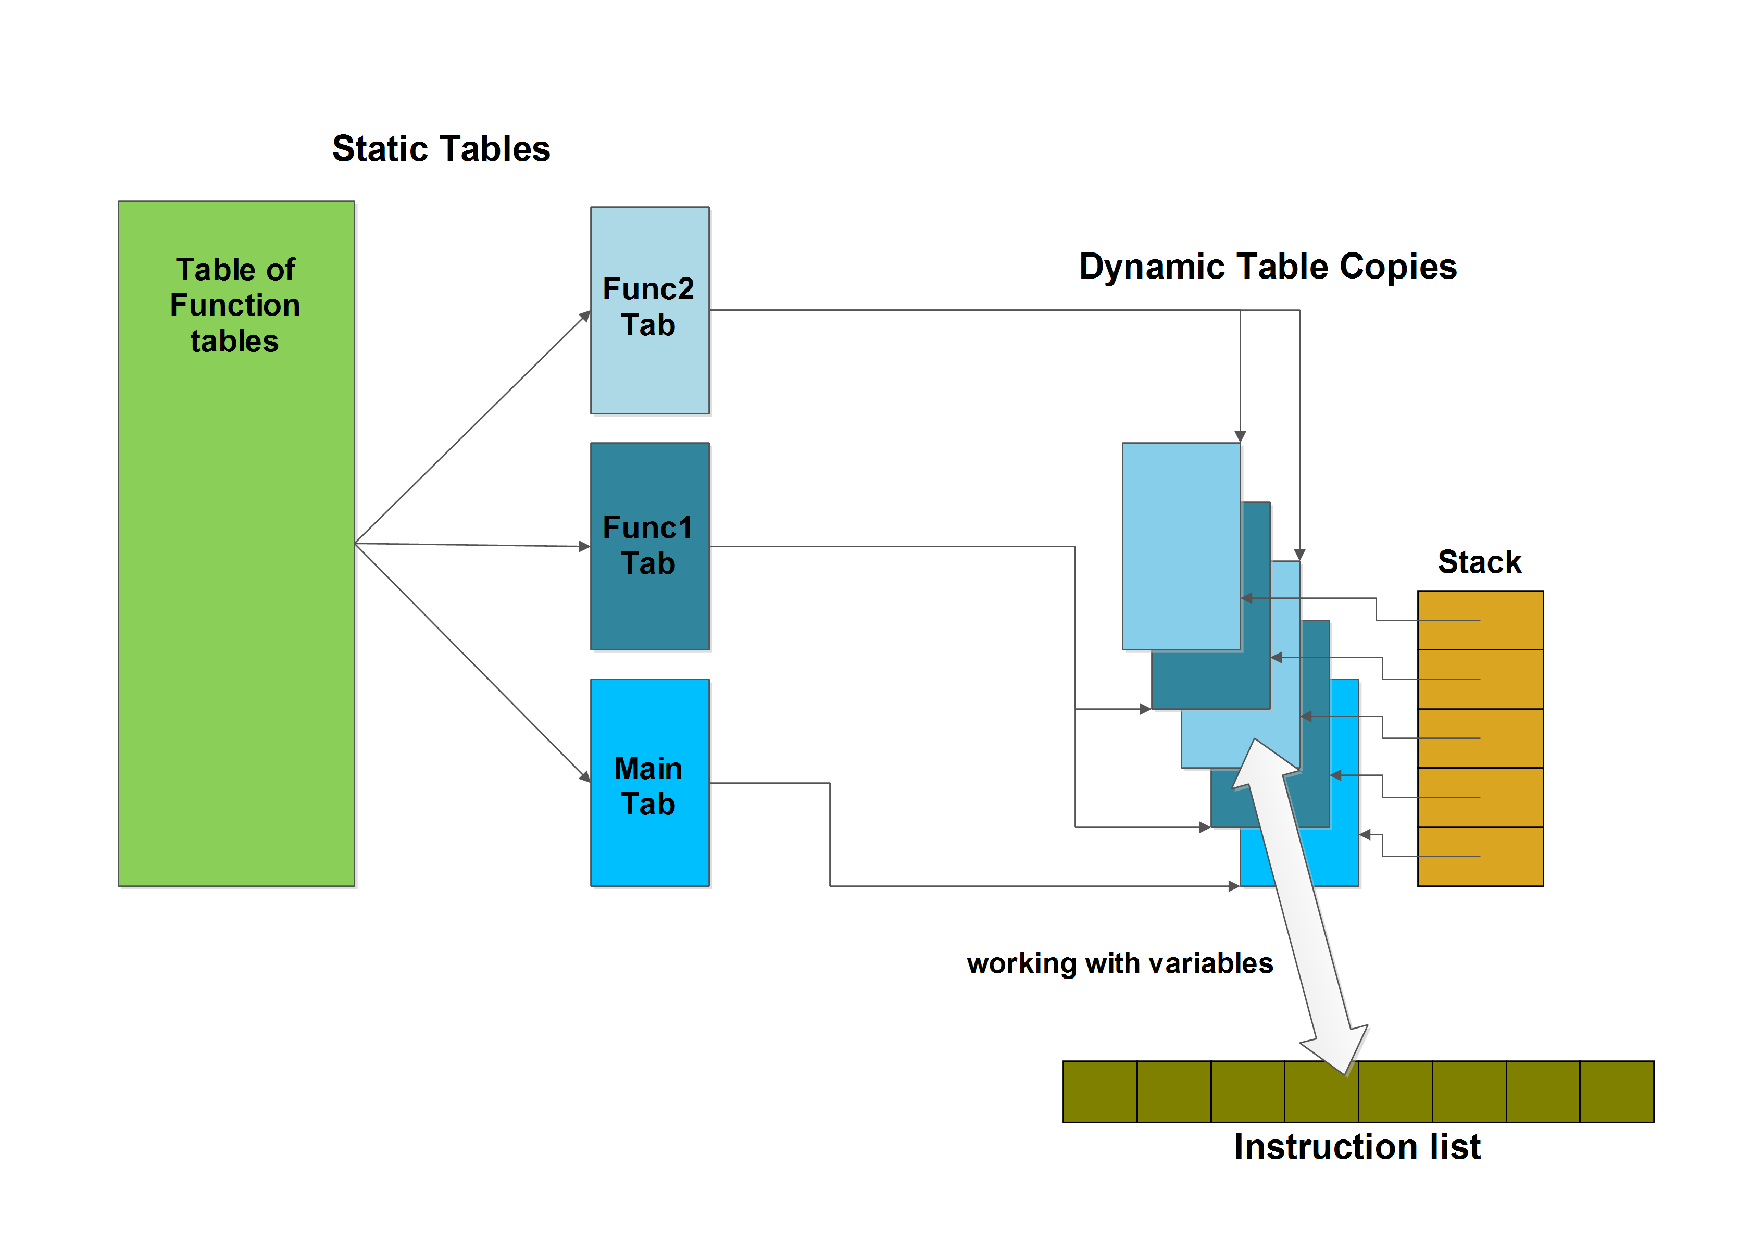
\includegraphics[trim=0 0 0 20px, scale=0.38]{tables.pdf}
  \end{center}
\end{frame}

\begin{frame}
  \begin{center}
  {\LARGE Děkujeme za pozornost.}
  \end{center}
\end{frame}

\end{document}
